% \begin{document}
\chapter{Programmazione Lineare}
\section{Geometria della PL}
Ci concentriamo su algoritmi \textit{senza} vincoli di iterezza. Come accennato in precedenza, questi sono piu' facili da risolvere rispetto alle varianti intere dato che, anche se l'insieme di soluzioni e' infinito, e' possibile guardare le caratterisctiche geometriche delle soluzioni ammissibili in modo da non dover guardarle tutte, ma solo alcune principali.

I vincoli lineari definiscono un'"area" di soluzioni ammissibili, che sara' definita da un poliedro (che puo' anche essere infinito) in quanto i vincoli sono lineari. Anche la funzione obbiettivo e' lineare, quindi guardando ogni valore che puo' assumere, forma una "retta" che puo' intersecare la regione ammissibile. L'ultima retta che forma la funzione obbiettivo che interseca quest'area (che ha quindi il valore ottimo) interseca per forza uno dei vertici che la delimitano.

Quindi ci basta controllare il valore della FO ai vertici per decidere. Ovviamente, il piano non e' per forza bidimensionale, quindi questa intuizione ci abbandona quando abbiamo piu' variabili. Dobbiamo dimostrarlo quindi usando la MATEMATICA

\subsection{Nozioni Preliminari}
Natura matriciale di oggetti geometrici in piu' dimensioni

  \subsubsection{Iperpiano}
  \dfn{\textbf{Iperpiano}}{
  si definisce \textbf{iperpiano} l'insieme $ \{x \in \mathbb{R}^{n} | a x = b\} $ con $ a \in \mathbb{R}^{n} $ e $ b \in \mathbb{R} $
  }

  \subsubsection{Semispazio}
  \dfn{\textbf{Semispazio}}{
    si definisce \textbf{semispazio} l'insieme $ \{x \in \mathbb{R}^{n} | a x \leq b\} $ con $ a \in \mathbb{R}^{n} $ e $ b \in \mathbb{R} $
  }
  Si può quindi facilmente concludere che l'iperpiano è il confine di un semispazio

  \subsubsection{Poliedro}
  intersezione $P$ di un numero finito di semispazi
  
  Formalmente:
  \dfn{\textbf{Poliedro}}{
    si definisce \textbf{poliedro} l'insieme $ P = \{x \in \mathbb{R}^{n} | Ax \leq b\} $ con $ A \in \mathbb{R}^{m \times n} $ e $ b \in \mathbb{R}^{m} $
  }

  \subsubsection{Insieme Convesso}
  l'insieme convesso è un insieme dove se io prendo due punti, la retta che li unisce è contenuta nell'insieme
  
  Formalmente:
  \dfn{\textbf{Insieme Convesso}}{
    si definisce \textbf{insieme convesso} l'insieme $ C \subseteq \mathbb{R}^{n} $ tale che $ \forall x\in C, \forall y \in C $ e $ \lambda \in [0,1] $ si ha che $ \lambda x + (1-\lambda)y \in C $
  }
  ne fanno parte tutti i poliedri e i semispazi

\subsubsection{Notazioni sui poliedri}
Sia un poliedro $ P = \{x \in \mathbb{R}^{n} | Ax \leq b\} $ e sia con $A\in\mathbb{R}^{m \times n}$ e $b\in\mathbb{R}^{m}$ e sia $I\subseteq \{1,...,m\} $ un qualunque sottoinsieme. Si denota:
\begin{itemize}
  \item $\overline{I} = \{1,...,m\} \setminus I$ il complemento di $I$
  \item $A_I$ la matrice $A$ formata dalle righe di $A$ considerando solo le righe $i\in I$
  \item $P_I$ il poliedro $P$ definito da $A_I$ e $b_I$ (cioe' le righe di $b$ corrispondenti a $I$), cioè:
  \[
    P_I = \{x \in \mathbb{R}^{n} | A_I x  = b_I \land A_{\overline{I}x}\leq b_{\overline{I}}\}
  \]
  In altre parole, $P_I$ è il poliedro definito dalle righe di $A$ e $b$ che sono in $I$, e le righe di $A$ e $b$ che non sono in $I$ sono considerate come vincoli di disuguaglianza
\end{itemize}
\subsection{Faccia}
\dfn{Faccia}{
  Sia $ P = \{x \in \mathbb{R}^{n} | Ax \leq b\} $ un poliedro e sia $I\subseteq \{1,...,m\}$ un qualunque sottoinsieme non vuoto. . Si definisce \textbf{faccia} di $ P $ l'insieme $P_I$ deifito sopra
}
Con questa definizione, piuttosto astratta, si può facilmente intuire che
\nt{
  il poliedro $P$ è una faccia di se stesso, e che ogni faccia di $P$ è un poliedro
}
si noti inoltre tale proposizione:
\mprop{Cardinalità dell'insieme delle facce di un poliedro}{
  Sia $ P = \{x \in \mathbb{R}^{n} | Ax \leq b\} $ un poliedro e sia $I\subseteq \{1,...,m\}$ un qualunque sottoinsieme non vuoto. Allora l'insieme delle facce di $P$ è finito e ha cardinalità al più $2^m$
}
\pf{Dimostrazione}{
  Ogni faccia di $P$ è definita da un sottoinsieme di $I \subseteq {1,\dots, m}$, pertanto la quantità di facce sarà al più quanto il numero di sottoinsiemi di $I$, ovvero l'inseme delle parti di $I$, che ha cardinalità $2^m$
  
}

Qui abbiamo due cose importanti:
\dfn{Faccia propria}{
  Sia $F$ una faccia di un poliedro $P$. Si dice \textbf{faccia propria} se $F \neq P$ e $F \neq \emptyset$
}

\dfn{Faccia massimale}{
  Sia $F$ una faccia di un poliedro $P$. Si dice \textbf{faccia massimale} se $\nexists F':F' \subset F$ e $F' \neq F$
}

Adesso introduco la nozione di di faccetta
\dfn{Faccetta}{
  Si definisce \textbf{faccetta} di un poliedro $P$ una $F$ sia propria che massimale
}


\dfn{Dimensione di una faccia}{
  La \textbf{dimensione} di una faccia $F$ di un poliedro $P$ è definita come la dimensione del più piccolo sottospazio che la contenga
}

\subsubsection{Vertici}

\mprop{Dimensione delle facce}{\label{prop:dimensione_faccia}
  Una faccia determinata da una matrice $A_I$ di rango $k$ ha dimensione $n - k$ o inferiore
}
\pf{Dimostrazione}{
  Sia data per esercizio al Basta
}

Da qui discende la definizione di vertice

\dfn{Vertice}{ \label{def:vertice}
  Si definisce \textbf{vertice} di un poliedro $P$ le facce individuate da matrici $A_I$ di rango $n$, ovvero le facce di dimensione $0$
}

\nt{
  Si noti che per \ref{prop:dimensione_faccia} e per \ref{def:vertice} l’equazione
  $A_I x = b_I$ ammette una e una sola soluzione
  
}
\subsubsection{Spigoli}
\dfn{Spigoli}{
  Si definisce \textbf{spigolo} di un poliedro $P$ l'insieme di punti che sono vertici di $P$ e che appartengono a facce di dimensione $1$, quindi definite da matrici $A_I$ di rango $n-1$
}

\subsection{Base}
\dfn{Base}{
  Si definisce \textbf{base} di un poliedro $P$ il sottorinsieme $B\subseteq {1,\dots, m}$ tale che $A_B$ è una matrice di rango massimo, ovvero $A_B$ è quadrata e invertibile. LA matrice $A_B$, inoltre, è detta \textbf{matrice di base} e $x_B = A^{-1}_B b_B$ è detta soluzione di base
}

\ex{Esempio numerico di base}{
  todo
}
Altra definizione importante è quella di \textbf{soluzione ammissibile} che è un punto che soddisfa i vincoli del poliedro, quindi $Ax \leq b$

\dfn{soluzione ammissibile}{
  Si definisce \textbf{soluzione ammissibile} di un poliedro $P$ una soluzione di base $x_B$ tale che $x_B\in P$
}

\subsection{Vincoli attivi}

Un concetto importante è quello di vincolo attivo, che è un vincolo che "limita" il poliedro, ovvero che lo definisce. Un vincolo attivo è un vincolo che è soddisfatto con uguaglianza in un punto ammissibile. Formalmente

\dfn{Vincolo attivo}{
  Sia $x_0\in P$, si definisce \textbf{vincolo attivo} in $x_0$ il vincolo $a_ix\leq b_i$ tale che $a_ix_0 = b_i$
}

Si denota con $I(x_0)$ l'insieme degli indici dei vincoli attivi in $x_0$
\dfn{Insieme degli indici dei vincoli attivi}{
  Sia $x_0\in P$, si definisce \textbf{insieme degli indici dei vincoli attivi} in $x_0$ l'insieme \[I(x_0) = \{i \mid a_ix_0 = b_i\}\]
}

Teoremino

\thm{Teorema Morbidelli}{
  Sia $P = \{x \in \mathbb{R}^{n} | Ax \leq b\} $ un poliedro, sia $x\in P$ una soluzione ammissibile e sia $I(x)$ l'insieme degli indici dei vincoli attivi in $x$
  \[
    \forall J\subseteq I(x) \quad P_J \text{ è una faccia di } P
  \]

  Inoltre $P_{I(x)}$ è una faccia minimale (ovvero la faccia più piccola che contiene $x$) tra tutte le facce $P_J$
}
\pf{Dimostrazione}{
  $\dots$
}


\section{Inviluppi Convessi}
Fino a questo punto del capitolo, i poliedri sono stati rappresentati attraverso le loro facce, ovvero come insiemi di vincoli lineari nello spazio. Ora introduciamo una rappresentazione alternativa: quella basata sui punti. In questa rappresentazione, il poliedro viene costruito a partire dai suoi vertici.

L'obiettivo è determinare il poliedro più piccolo che contenga un dato insieme di punti, i quali non necessariamente coincidono con i vertici. I punti sono rappresentati come vettori in uno spazio n-dimensionale, e il poliedro viene costruito considerando tutte le combinazioni lineari con coefficienti non negativi che sommano a uno. In altre parole, si tratta di una media pesata dei punti, dove i pesi sono positivi e la loro somma è pari a uno.

L'insieme ottenuto in questo modo è chiamato \textbf{inviluppo convesso} dei punti dati. Esso rappresenta il poliedro più piccolo che contiene tutti i punti considerati.

Formalmente ecco la definizione di inviluppo convesso:
\dfn{
  Inviluppo convesso
}{
  Sia $X = \{x_1,\dots,x_k\} \subseteq \mathbb{R}^{n}$ un insieme di punti. Si definisce \textbf{inviluppo convesso} di $X$ l'insieme
  \[
    \text{conv}(X) = \left\{ x = \sum_{i=1}^{s} \lambda_i x_i \mid \sum_{i=1}^{s} \lambda_i = 1 \land \lambda_i \geq 0 \right\}
  \]
}

  \mprop{}{
    Sia $X = \{x_1, \dots, x_k\} \subseteq \mathbb{R}^n$. L'inviluppo convesso $\text{conv}(X)$ è il più piccolo insieme convesso che contiene tutti i punti di $X$
  }

  \dfn{politopo}{
    Si definisce \textbf{politopo} un poliedro limitato i cui vertici appartengono all'insieme $X$
  }
  \clm{}{}{
      Sia $X = \{x_1, \dots, x_k\} \subseteq \mathbb{R}^n$. Allora $\text{conv}(X)$ è un politopo.
  }
\ex{}{
  L'inviluppo convesso dei seguenti punti
\begin{center}
  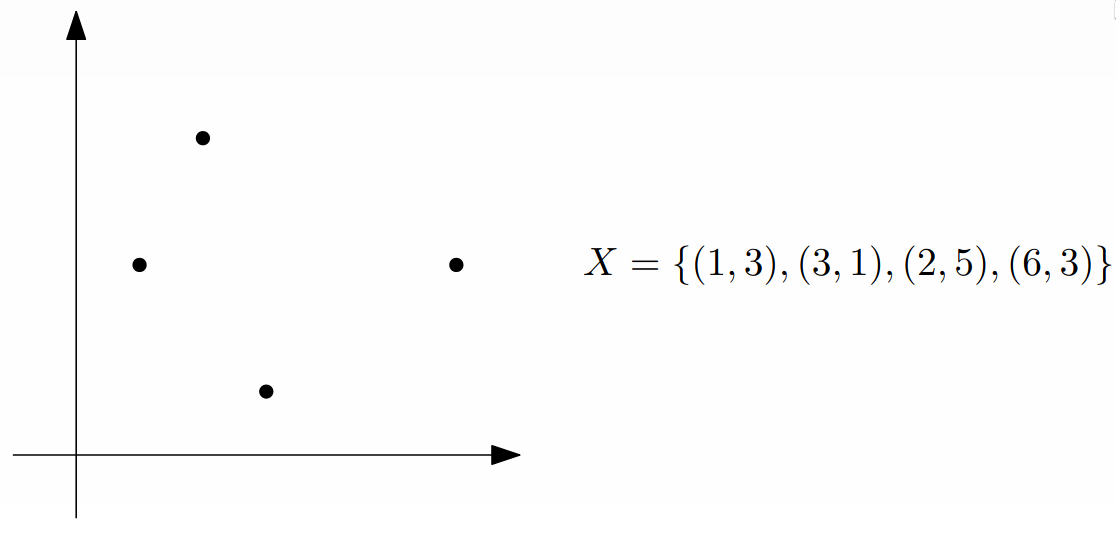
\includegraphics[width=0.5\textwidth]{img/2025-04-14-09-43-27.png}
\end{center}
E' il quadrilatero che ha i punti come vertici. Ha fatto un discorso con triangoli e piani, va beh viene questo:
\begin{center}
  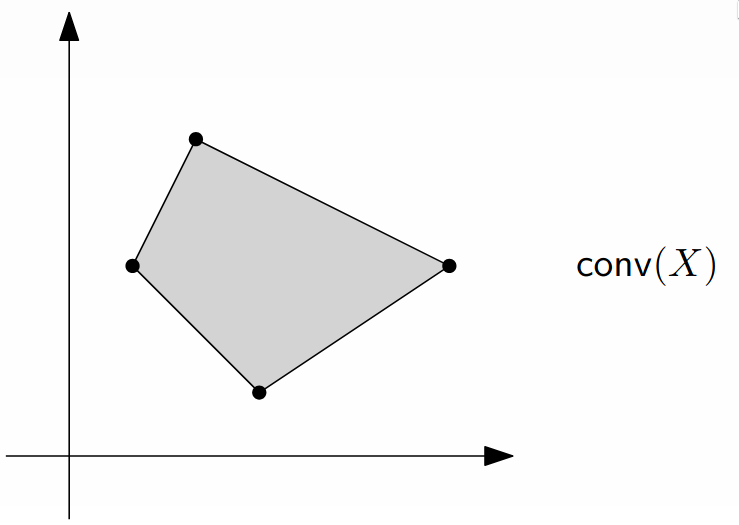
\includegraphics[width=0.5\textwidth]{img/2025-04-14-09-45-25.png}
\end{center}
}

\nt{
  E' possibile che un punto non faccia parte dei vertici, ma che sia un punto interno. Infatti, se nell'esempio di prima mettessimo un punto al centro, l'inviluppo convesso non cambierebbe.
}

\subsection{Coni Convessi}

\dfn{Cono}{
  Si definisce \textbf{cono} l'insieme $C\subseteq \mathbb{R}^n$ tale che
  \[
    \forall x \in C, \forall \alpha \in \mathbb{R}^+ \quad \alpha x \in C
  \]
}

Da cui discende la definizione di cono convesso, che è un cono che contiene anche l'origine
\dfn{Cono convesso}{
  Si definisce \textbf{cono convesso} l'insieme un cono $C\subseteq \mathbb{R}$ tali che
  \[
    \forall x,y\in C, \forall \lambda, \mu\in \mathbb{R} \implies \lambda x + \mu y \in C
  \]
}

Esiste tuttavia una definizione basata sulle direzione (ovvero vettori di punti)

\dfn{cono finitamente generato}{
  Dato un insieme $V = \{v_1, \dots, v_k\} \subset \mathbb{R}^n$, si definisce \textbf{cono finitamente generato} da $V$ l'insieme
  \[
  \text{cono}(V) = \left\{ v = \sum_{i=1}^{k} \nu_i v_i \mid \nu_i \geq 0 \right\}
  \]
}
\mprop{}{
  L'insieme $\text{cono}(V)$ è il più piccolo cono convesso che contiene tutti i vettori di $V$
}

Si noti l'esempio di cono convesso:
\ex{Esempio visuale del cono convesso}{
  Si parte dai seguenti punti
  \begin{center}
    \includegraphics[width=0.5\textwidth]{img/inisieme_X_iniziale_per_il_cono.png}
  \end{center}
  Il cono convesso generato da questi punti non è altro che
  \begin{center}
    \includegraphics[width=0.5\textwidth]{img/cono_convesso_di_X.png}
  \end{center}
}

\subsection{Teorema di Motzkin}
Operazione che codifica l'intuizione che i concetti di coni e inviluppi hanno a che fare con i poliedri. Il cono convesso cattura il concetto di possibile illimitatezza, quindi mescoliamo le due cose usando le somme fra insiemi di vettori.

Bho okay buon alex

\thm{Teorema di Motzkin}{   \label{thm:motzkin}
  $ P \subseteq \mathbb{R}^{n} $ e' un poliedro sse esistono $ X,V $ finiti tali che $ P = conv(X) + cono(V) $
}
La cosa cruciale e' il legame fra il mondo di vincoli e quello di punti e direzioni. Non lo dimostriamo perche no.

\nt{
  Sta roba puo' sembrare ovvia in 2d, ma in dimensioni piu' alte non e' cosi ovvio ed e' per questo che e' tanta roba.
}

\subsection{Due Rappresentazioni}
All'aumentare delle dimensioni, i vertici aumentano in modo esponenziale $ 2^{n} $, mentre i vincoli aumentano molto piu' lentamente $ 2n $. Male male sta cosa, perche' noi siamo INFORMATICI (anche Ugo), e ci servono algoritmi rapidi.

\subsection{Teorema Fondamentale}
\thm{}{
  Sia $ P = \{x \mid Ax \leq b\} $ e siano $ x_1,\dots,x_s, v_1,\dots,v_t \in \mathbb{R}^{n} $ tali che
  \[
    P = conv(\{x_1,\dots,x_s\}) + cono(\{v_1,\dots,v_t\})
  \]
  Allora il problema $ \max{ \{cx \mid Ax \leq b\}} $ ha un ottimo finito sse $cv_j\leq 0 \forall j \in \{1,\dots, t\}$. In tal caso esiste un $k \in \{1,\dots,s\}$ tale che $x_k$ e' una soluzione ottima
}

\pf{Dimostrazione}{
  Per \ref{thm:motzkin} si ha che il problema $\max{\{ cx\mid Ax\leq b \}}$ è equivalente al seguente problema:
  \[
    \max{c\left( \sum_{i=1}^s\lambda_i x_i + \sum_{j=1}^{t} \nu_j v_j \right)} = \max{\sum_{i=1}^{s} \lambda_i (cx_i) + \sum_{j=1}^{t} \nu_j (cv_j)}
  \]
  Con $ \lambda_i \geq 0 $ e $ \nu_j \geq 0 $ e $ \sum_{i=1}^{s} \lambda_i = 1 $. 

  Tale problema ha ottimo finito sse $c\nu_j \leq 0$ per ogni $j \in {1,\dots , t}$. Infatti:
  \begin{itemize}
    \item $\Rightarrow$: se fosse $cv_j > 0$ per un certo $j$, allora $\nu_j$ potrebbe essere scelto arbitrariamente grande, e quindi la funzione obbiettivo divergerebbe
    \item $\Leftarrow$: Supponiamo che $cv_j \leq 0$ per ogni $j \in \{1, \ldots, t\}$, e prendiamo un $y \in P$. Abbiamo che, se $\lambda_i$ e $\nu_j$ sono i corrispondenti coefficienti del teorema di decomposizione,

    \[
    \begin{aligned}
          cy &= \sum_{i=1}^{s} \lambda_i (cx_i) + \sum_{j=1}^{t} \nu_j (cv_j)\\
          &\leq \sum_{i=1}^{s} \lambda_i (cx_i) \leq \sum_{i=1}^{s} \lambda_i (cx_k) = cx_k
    \end{aligned}
    \]
    
    dove $x_k$ è il vettore tale che $x_k = \max\{cx_i \mid i = 1, \ldots, s\}$. Quindi $x_k$ è una soluzione ottima finita.
    
  \end{itemize}
}

\nt{
  La condizione $ cv_j \leq 0 $ significa che andando verso le direzioni, la funzione da massimizzare decresce. Dato che le soluzioni ammissibili possono essere illimitate solo lungo queste direzioni, significa che la funzione obbiettivo non puo' aumentare illimitatamente.
  }

  


\section{Dualità}

La \textbf{teoria della dualità} è  una branca dell'algebra lineare che studia le relazioni tra problemi di ottimizzazione. Si basa sull'udea che ad ogni problema di PL (chiamato \textbf{primale}) è associato mediante una funzione detta \textbf{involuzione} un altro problema (chiamato \textbf{duale}) che ha una struttra simile. Applicando l'involuzione al problema duale si ottiene il problema primale. 

\subsection{Coppie di problemi}
\dfn{Coppia di problemi}{
  Si definisce \textbf{coppia di problemi} la coppia di problemi
  \[
    \begin{aligned}
      \text{primale:} & \quad \max{cx} \\
      & \quad Ax \leq b\\
      & \quad x\geq 0\\
      \text{duale:} & \quad \min{by}\\
      & \quad A^Ty = c\\
      & \quad y\geq 0
    \end{aligned}
  \]
}

Qui verranno presentate le coppie simmetriche e quelle asimmetriche in maniera approssimativa
\subsubsection{Coppie asimmetriche}
\dfn{
  Coppia asimmetriche
}{
  Si definisce \textbf{coppia asimmetrica} la coppia di problemi
  \[
    \begin{aligned}
      \text{primale:} &\quad \max{cx\mid (Ax \leq b) \land (x\geq 0)} \\
      \text{duale:} &\quad \min{yb\mid (yA = c) \land (y\geq 0)}\\
    \end{aligned}
  \]
}

\subsubsection{Coppie simmetriche}
\dfn{Coppia simmetrica}{ \label{def:coppia_simmetrica}
  Si definisce \textbf{coppia simmetrica} la coppia di problemi
  \[
    \begin{aligned}
      \text{primale:} & \quad \max{\{cx \mid Ax \leq b\}} \\
      \text{duale:} & \quad \min{\{yb \mid (yA = c) \land (y \geq 0)\}}\\
    \end{aligned}
  \]
}

\subsection{Teoremi sualla dualità}

\subsubsection{Teorema del duale del duale}

\mlenma{}{ \label{lem:minmax}
  Per qualsiasi funzione $f(y)$ e per qualsiasi insieme ammissibile $S$ su cui $f(y)$ è definita, vale la seguente relazione:
  \[
  \min{\{f(y) \mid y \in S\}} = -\max{\{-f(y) \mid y \in S\}}
  \]
}

\pf{Dimostrazione}{
  Sia $f(y)$ una funzione definita su un insieme ammissibile $S$. Minimizzare $f(y)$ equvale a trovare un $v_m\leq f(y)\,\forall y\in S$, invece massimizzare $-f(y)$ equivale a trovare un $v_M\geq -f(y)\,\forall y\in S$, moltiplicando per $-1$ si ha che $-v_M\leq f(y)\,\forall y\in S$.
}

\thm{sul duale del duale}{
  Sia $P$ un problema primale e sia $D$ il suo duale. Allora $D$ è il duale di $P$ e $P$ è il duale di $D$

  \begin{center}
    
    \includegraphics[width=10cm]{img/duale_primale.png}
  \end{center}
}
\pf{
  Dimostrazione nel caso della coppia simmetriche
}{
  È possibile esprimere il duale della coppia simmetrica per \ref{lem:minmax} e \ref{def:coppia_simmetrica}:
  \[
    \begin{aligned}
      &-\max{\{ -yb \mid (yA\geq c) \land (y\geq 0) \}}=\\
      &-\max{\{ (-b^T)y \mid ((-A^T)y \leq -c) \land (y\leq 0) \}}\\
    \end{aligned}
  \]
  Il cui duale è
  \[
    \begin{aligned}
      &-\min{\{ -xc \mid (x(-A^T) \geq -b) \land (x\geq 0) \}}=\\
      &\max{\{ cx \mid Ax\leq b \land x\geq 0 \}}\\
    \end{aligned}\]
}

\subsubsection{Teorema Debole di Dualità}
\thm{Teorema Debole di Dualità}{  \label{thm:teorema_debole_di_dualita}
  Siano $\overline{x}$ e $\overline{y}$ rispettivamente una soluzione ammissibile del problema primale e del problema duale. Allora vale la seguente disuguaglianza:
  \[
    c\overline{x} \leq b\overline{y}
  \]
}
\pf{Dimostrazione nel caso della coppia asimmetrica}{
    \[
      \begin{cases}
        A\overline{x} \leq b \\
        \overline{y}A = c \\
        \overline{y} \geq 0
      \end{cases}\implies
      \begin{cases}
        \overline{y}A\overline{x} \leq \overline{y} b \\
        \overline{y}A\overline{x} = c\overline{x} \\
        \overline{y} \geq 0 \\
      \end{cases}\implies
      c\overline{x} \leq b\overline{y}
    \]
}

\pf{Nel caso di coppia simmetrica}{
  \[
    \begin{cases}
      A\overline{x} \leq b \\
      \overline{y}A \geq c \\
      \overline{y} \geq 0\\
      \overline{x} \geq 0
    \end{cases}\implies
    \begin{cases}
      \overline{y}A\overline{x} \leq \overline{y} b \\
      \overline{y}A\overline{x} \geq c\overline{x} \\
      \overline{y} \geq 0 \\
      \overline{x} \geq 0
    \end{cases}\implies
    c\overline{x} \leq b\overline{y}
  \]
}

\cor{Illimitatezza del primale e duale vuoto}{
  Se il problema primale è illimitato, allora il problema duale è vuoto. Viceversa, se il problema duale è vuoto, allora il problema primale è illimitato.
}
\pf{Dimostrazione}{
  Se il problema primale è illimitato, allora 
  \[
    \forall M\in \mathbb{R}\,\exists \overline{x}\in P :cx > M
  \]
  Poniamo per assurdo che $\exists \overline{y}$ soluzione ammissibile del duale. Allora, per la precedenze deduzione, si ha che
  \[
    \exists \overline{x} \in P : c\overline{x} > b\overline{y}
  \]
  Tuttavia per \ref{thm:teorema_debole_di_dualita} si ha una contraddizione
}

\cor{
  sulle soluzioni ottime
}{
  Siano $\overline{x}$ e $\overline{y}$ rispettivamente soluzioni ammissibili per il problema primale e per il problema duale e valga la seguente uguaglianza:
  \[
    c\overline{x} = b\overline{y}
  \]
  Allora $\overline{x}$ e $\overline{y}$ sono soluzioni ottime
}
\pf{Dimostrazione}{
  Sia $c\overline{x} = b\overline{y}$. Assumiamo per assurdo che $\overline{x}$ non sia una soluzione ottima. Allora esiste un $z$ ammissibile per il primale tale che $cz >\overline{y}b$, ma per \ref{thm:teorema_debole_di_dualita} si ha uan contraddizione
}
\subsection{Direzioni ammissibili}

È lecito chiedersi se, data una coppia assimetrica e considerato un $\overline{x}$ soluzione ammissibile per il primale, spostando $\overline{x}$ lungo una direzione dell'iperspazio, si ottiene o meno una nuova soluzione ammissibile. Ebbene ci si sta chiedendo se esiste la cosidetta direzione ammissibile

\dfn{Direzione ammissibile}{
  Si definisce \textbf{direzione ammissibile} un vettore $\xi$ sse
  \[
    \exists \overline{\lambda} >0 : x ( \lambda) = \overline{x} + \lambda \xi 
  \]
  Dove x($\lambda$) è ammissibile nel primale $\forall \lambda\in [0,\overline{\lambda}]$
}

\mlenma{sull'ammissibilità del vettore direzione}{
  il vettore $\xi$ è direzione ammissibile per $\overline{x}$ sse
  \[
    A_{I(\overline{x})} \xi \leq 0
  \]
}

\pf{Dimostrazione}{
  Devo dimostrare che
  \[
    \forall i\in\{1,\dots, m\}\quad A_{i}x(\lambda)=A_{i}\overline{x} +\lambda A_{i}\xi \leq b_{i}
  \]
  Si ha che 
  \begin{itemize}
    \item se $i\in I(\overline{x})$, allora $A_{i}\overline{x} = b_{i}$ pertanto l'quazione è verificata sse $\lambda A_{i}\xi \leq 0$
    \item se $i\notin I(\overline{x})$, allora $A_{i}\overline{x} < b_{i}$ pertanto l'quazione è verificata sse $\lambda A_{i}\xi \leq b_{i} - A_{i}\overline{x}$ e dato che $b_{i} - A_{i}\overline{x}\geq 0$ l'equazione è sicuramente verificata se $\lambda A_{i}\xi \leq 0$
  \end{itemize}
}

\subsection{Direzione di crescita}
\dfn{Direzione di crescita}{
  Si definisce \textbf{direzione di crescita} per $\overline{x}$ un vettore direzione $\xi\in \mathbb{R}^n$ se
  \[
    \exists \lambda : cx(\lambda) = c\overline{x} + \lambda c\xi > c\overline{x} \iff c\xi > 0
  \]
  Ossia se uno spostamento lungo la direzione $\xi$ porta ad un incremento della funzione obbiettivo
}

si osservi che 
\nt{
  \begin{itemize}
    \item se $c=0$ la funzione obbiettivo è sempre zero, quindi tutte le soluzioni ammissibili sono ottime
    \item se $c\neq 0$ allora se esiste una direzione ammissibile per $\overline{x}$ che sia anche di crescita, allora $\overline{x}$ non può essere ottimo.
  \end{itemize}
}